\documentclass[a4paper]{report}
% Some basic packages
\usepackage[utf8]{inputenc}
\usepackage[T1]{fontenc}
\usepackage{textcomp}
\usepackage[english]{babel}
\usepackage{url}
\usepackage{graphicx}
\usepackage{float}
\usepackage{booktabs}
\usepackage{enumitem}

\pdfminorversion=7

% Don't indent paragraphs, leave some space between them
\usepackage{parskip}

% Hide page number when page is empty
\usepackage{emptypage}
\usepackage{subcaption}
\usepackage{multicol}
\usepackage{xcolor}

% Other font I sometimes use.
% \usepackage{cmbright}

% Math stuff
\usepackage{amsmath, amsfonts, mathtools, amsthm, amssymb}
% Fancy script capitals
\usepackage{mathrsfs}
\usepackage{cancel}
% Bold math
\usepackage{bm}
% Some shortcuts
\newcommand\N{\ensuremath{\mathbb{N}}}
\newcommand\R{\ensuremath{\mathbb{R}}}
\newcommand\Z{\ensuremath{\mathbb{Z}}}
\renewcommand\O{\ensuremath{\emptyset}}
\newcommand\Q{\ensuremath{\mathbb{Q}}}
\newcommand\C{\ensuremath{\mathbb{C}}}
\renewcommand\L{\ensuremath{\mathcal{L}}}

% Package for Petri Net drawing
\usepackage[version=0.96]{pgf}
\usepackage{tikz}
\usetikzlibrary{arrows,shapes,automata,petri}
\usepackage{tikzit}
\input{petri_nets_style.tikzstyles}

% Easily typeset systems of equations (French package)
\usepackage{systeme}

% Put x \to \infty below \lim
\let\svlim\lim\def\lim{\svlim\limits}

%Make implies and impliedby shorter
\let\implies\Rightarrow
\let\impliedby\Leftarrow
\let\iff\Leftrightarrow
\let\epsilon\varepsilon

% Add \contra symbol to denote contradiction
\usepackage{stmaryrd} % for \lightning
\newcommand\contra{\scalebox{1.5}{$\lightning$}}

% \let\phi\varphi

% Command for short corrections
% Usage: 1+1=\correct{3}{2}

\definecolor{correct}{HTML}{009900}
\newcommand\correct[2]{\ensuremath{\:}{\color{red}{#1}}\ensuremath{\to }{\color{correct}{#2}}\ensuremath{\:}}
\newcommand\green[1]{{\color{correct}{#1}}}

% horizontal rule
\newcommand\hr{
    \noindent\rule[0.5ex]{\linewidth}{0.5pt}
}

% hide parts
\newcommand\hide[1]{}

% si unitx
\usepackage{siunitx}
\sisetup{locale = FR}

% Environments
\makeatother
% For box around Definition, Theorem, \ldots
\usepackage{mdframed}
\mdfsetup{skipabove=1em,skipbelow=0em}
\theoremstyle{definition}
\newmdtheoremenv[nobreak=true]{definitie}{Definitie}
\newmdtheoremenv[nobreak=true]{eigenschap}{Eigenschap}
\newmdtheoremenv[nobreak=true]{gevolg}{Gevolg}
\newmdtheoremenv[nobreak=true]{lemma}{Lemma}
\newmdtheoremenv[nobreak=true]{propositie}{Propositie}
\newmdtheoremenv[nobreak=true]{stelling}{Stelling}
\newmdtheoremenv[nobreak=true]{wet}{Wet}
\newmdtheoremenv[nobreak=true]{postulaat}{Postulaat}
\newmdtheoremenv{conclusie}{Conclusie}
\newmdtheoremenv{toemaatje}{Toemaatje}
\newmdtheoremenv{vermoeden}{Vermoeden}
\newtheorem*{herhaling}{Herhaling}
\newtheorem*{intermezzo}{Intermezzo}
\newtheorem*{notatie}{Notatie}
\newtheorem*{observatie}{Observatie}
\newtheorem*{exe}{Exercise}
\newtheorem*{opmerking}{Opmerking}
\newtheorem*{praktisch}{Praktisch}
\newtheorem*{probleem}{Probleem}
\newtheorem*{terminologie}{Terminologie}
\newtheorem*{toepassing}{Toepassing}
\newtheorem*{uovt}{UOVT}
\newtheorem*{vb}{Voorbeeld}
\newtheorem*{vraag}{Vraag}

\newmdtheoremenv[nobreak=true]{definition}{Definition}
\newtheorem*{eg}{Example}
\newtheorem*{notation}{Notation}
\newtheorem*{previouslyseen}{As previously seen}
\newtheorem*{remark}{Remark}
\newtheorem*{note}{Note}
\newtheorem*{problem}{Problem}
\newtheorem*{observe}{Observe}
\newtheorem*{property}{Property}
\newtheorem*{intuition}{Intuition}
\newmdtheoremenv[nobreak=true]{prop}{Proposition}
\newmdtheoremenv[nobreak=true]{theorem}{Theorem}
\newmdtheoremenv[nobreak=true]{corollary}{Corollary}

% End example and intermezzo environments with a small diamond (just like proof
% environments end with a small square)
\usepackage{etoolbox}
\AtEndEnvironment{vb}{\null\hfill$\diamond$}%
\AtEndEnvironment{intermezzo}{\null\hfill$\diamond$}%
% \AtEndEnvironment{opmerking}{\null\hfill$\diamond$}%

% Fix some spacing
% http://tex.stackexchange.com/questions/22119/how-can-i-change-the-spacing-before-theorems-with-amsthm
\makeatletter
\def\thm@space@setup{%
  \thm@preskip=\parskip \thm@postskip=0pt
}


% Exercise 
% Usage:
% \exercise{5}
% \subexercise{1}
% \subexercise{2}
% \subexercise{3}
% gives
% Exercise 5
%   Exercise 5.1
%   Exercise 5.2
%   Exercise 5.3
\newcommand{\exercise}[1]{%
    \def\@exercise{#1}%
    \subsection*{Exercise #1}
}

\newcommand{\subexercise}[1]{%
    \subsubsection*{Exercise \@exercise.#1}
}


% \lecture starts a new lecture (les in dutch)
%
% Usage:
% \lecture{1}{di 12 feb 2019 16:00}{Inleiding}
%
% This adds a section heading with the number / title of the lecture and a
% margin paragraph with the date.

% I use \dateparts here to hide the year (2019). This way, I can easily parse
% the date of each lecture unambiguously while still having a human-friendly
% short format printed to the pdf.

\usepackage{xifthen}
\def\testdateparts#1{\dateparts#1\relax}
\def\dateparts#1 #2 #3 #4 #5\relax{
    \marginpar{\small\textsf{\mbox{#1 #2 #3 #5}}}
}

\def\@lecture{}%
\newcommand{\lecture}[3]{
    \ifthenelse{\isempty{#3}}{%
        \def\@lecture{Lecture #1}%
    }{%
        \def\@lecture{Lecture #1: #3}%
    }%
    \subsection*{\@lecture}
    \marginpar{\small\textsf{\mbox{#2}}}
}



% These are the fancy headers
\usepackage{fancyhdr}
\pagestyle{fancy}

% LE: left even
% RO: right odd
% CE, CO: center even, center odd
% My name for when I print my lecture notes to use for an open book exam.
% \fancyhead[LE,RO]{Gilles Castel}

\fancyhead[RO,LE]{\@lecture} % Right odd,  Left even
\fancyhead[RE,LO]{}          % Right even, Left odd

\fancyfoot[RO,LE]{\thepage}  % Right odd,  Left even
\fancyfoot[RE,LO]{}          % Right even, Left odd
\fancyfoot[C]{\leftmark}     % Center

\makeatother




% Todonotes and inline notes in fancy boxes
\usepackage{todonotes}
\usepackage{tcolorbox}

% Make boxes breakable
\tcbuselibrary{breakable}

% Verbetering is correction in Dutch
% Usage: 
% \begin{verbetering}
%     Lorem ipsum dolor sit amet, consetetur sadipscing elitr, sed diam nonumy eirmod
%     tempor invidunt ut labore et dolore magna aliquyam erat, sed diam voluptua. At
%     vero eos et accusam et justo duo dolores et ea rebum. Stet clita kasd gubergren,
%     no sea takimata sanctus est Lorem ipsum dolor sit amet.
% \end{verbetering}
\newenvironment{verbetering}{\begin{tcolorbox}[
    arc=0mm,
    colback=white,
    colframe=green!60!black,
    title=Opmerking,
    fonttitle=\sffamily,
    breakable
]}{\end{tcolorbox}}

% Noot is note in Dutch. Same as 'verbetering' but color of box is different
\newenvironment{noot}[1]{\begin{tcolorbox}[
    arc=0mm,
    colback=white,
    colframe=white!60!black,
    title=#1,
    fonttitle=\sffamily,
    breakable
]}{\end{tcolorbox}}




% Figure support as explained in my blog post.
\usepackage{import}
\usepackage{xifthen}
\usepackage{pdfpages}
\usepackage{transparent}
\newcommand{\incfig}[1]{%
    \def\svgwidth{\columnwidth}
    \import{./figures/}{#1.pdf_tex}
}

% Fix some stuff
% %http://tex.stackexchange.com/questions/76273/multiple-pdfs-with-page-group-included-in-a-single-page-warning
\pdfsuppresswarningpagegroup=1


% My name
\author{Bruno M. Pacheco}

 
\begin{document}
 
\title{Laboratório 4}
\author{Bruno M. Pacheco (16100865)\\
Pedro Y. F. Ceripes (18100681) \\
EEL 7550 - Eletrônica Aplicada}
 
\maketitle

\section*{Objetivo}
 
Esse roteiro de experimentos visa desenvolver familiaridade com o uso de diodos através de modelos de componentes reais (1N4001) em arranjos comuns, demonstrados através dos 4 circuitos propostos.
 
\section*{Simulações}

\subsection*{Circuito 1}

Considerando o diodo ideal, o valor de pico na saída seria o mesmo da entrada, então $V_{o,p} = 10 V$. Já o valor médio da tensão de saída pode ser encontrado por \[
V_{o,med} = \frac{1}{T}\int_{0}^{T} \left| V_{o}\left( t \right)  \right| dt = \frac{1}{T}\left( \frac{T}{2}\cdot \frac{10}{2} \right) = 2,5\,V
.\] 

Considerando a aproximação do diodo com uma queda de tensão de $0,7\,V$, o valor de pico da saída simplesmente sofre a queda do diodo, i.e., $V_{o,p} = 10 - 0,7 = 9,3\, V$, enquanto o valor médio da tensão de saída pode ser aproximado por \[
V_{o,med} = \frac{1}{T}\int_{0}^{T} \left| V_{o}\left( t \right)  \right| dt \approx \frac{1}{T}\left( \frac{T}{2}\cdot \frac{V_{o,p}}{2} \right) = 2,325\,V
.\] 

Para o circuito implementado no LTSpice com o modelo do diodo 1N4001, a medição foi feita com ferramentas do LTSpice conforme na figura \ref{fig:figures-lab4-1-png}.

\begin{figure}[H]
    \centering
    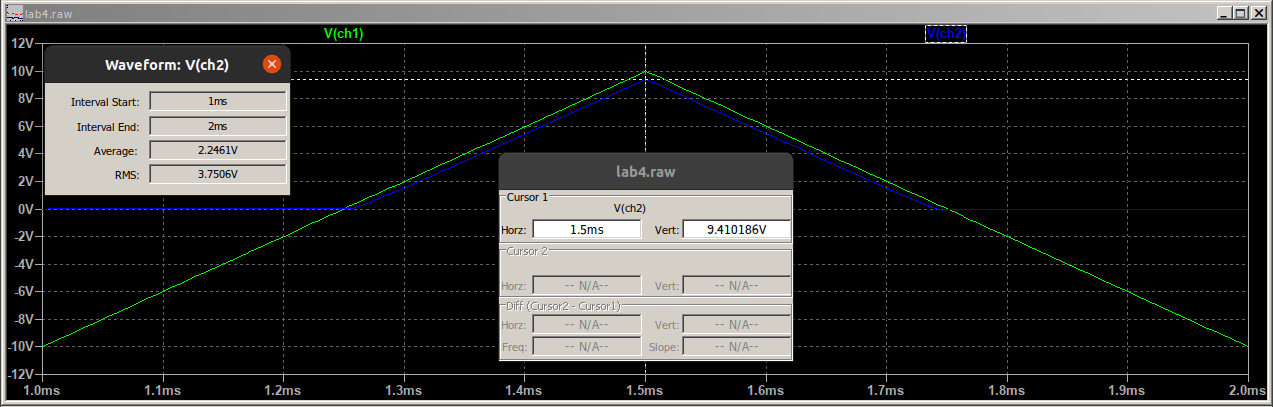
\includegraphics[width=0.8\textwidth]{figures/lab4-1.png}
    \caption{Medição realizada em $V_o$ utilizando as ferramentas do LTSpice.}
    \label{fig:figures-lab4-1-png}
\end{figure}

Os resultados medidos foram conforme na tabela abaixo.

\begin{table}[H]
    \centering
    \begin{tabular}{c | c}
	Medida & Resultado \\
	\hline
	$V_{i,p}$ & 9,98 V \\
	$V_{o,p}$ & 9,41 V \\
	$V_{i,med}$ & 0 V \\
	$V_{o,med}$ & 2,25 V
    \end{tabular}
\end{table}

Ainda que o valor de pico da tensão de saída seja maior na simulação do que na aproximação feita para o diodo não ideal, o valor médio encontrado é inferior. Isso é esperado uma vez que a aproximação feita considera que a saída no semiciclo positivo é sempre proporcional à entrada, o que não é verdade pois há um atraso até que a tensão de entrada supere a tensão de condução do diodo.

\subsection{Circuito 2}

Para calcular o valor teórico de $\Delta V_o$, utilizaremos a equação simplificada \ref{eq:exe2}. Vale ressaltar que para facilitar a visualização dos valores, a fonte foi iniciada em 10V.

\begin{equation}
    \label{eq:exe2}
    \Delta V_o = \frac{V_p}{C_1R_1f} = \frac{10}{10k \cdot 1\mu \cdot 1k} = 1V
\end{equation}

Após isso foi montado o circuito no software LTspice, como mostrado na figura \ref{fig:figures-lab4-2-circuito-png}.

\begin{figure}[H]
    \centering
    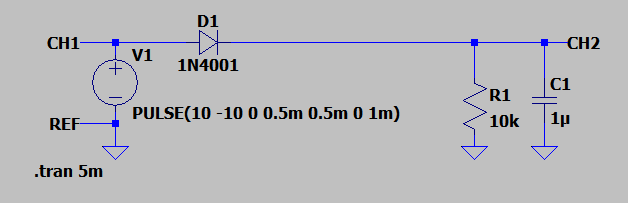
\includegraphics[width=0.8\textwidth]{figures/lab4-2-circuito.PNG}
    \caption{Segundo circuito simulado no LTSpice.}
    \label{fig:figures-lab4-2-circuito-png}
\end{figure}

Sendo assim, o circuito foi simulado com resultado apresentado no gráfico mostrado na figura \ref{fig:figures-lab4-2-grafico-png}.

\begin{figure}[H]
    \centering
    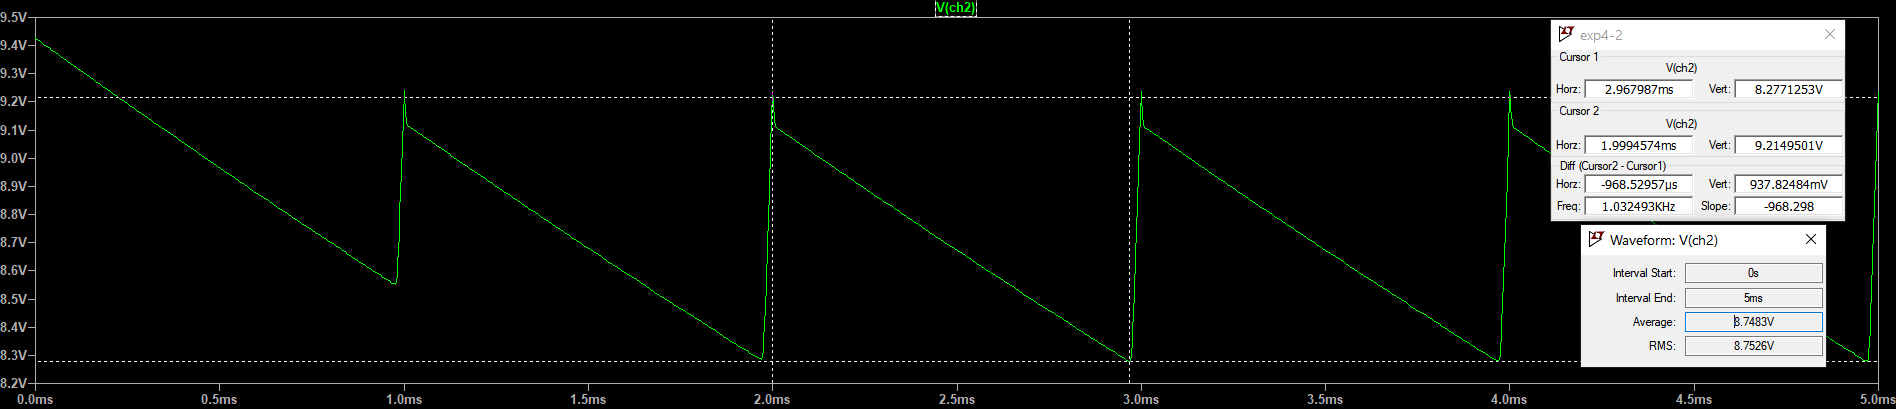
\includegraphics[width=0.8\textwidth]{figures/lab4-2-grafico.PNG}
    \caption{Resposta de $V_o$ no tempo na simulação do LTspice.}
    \label{fig:figures-lab4-2-grafico-png}
\end{figure}

Pelo gráfico acima percebemos que $\Delta V_o = 0.937V \approx 1V$ e que $V_{o,med} \approx 8.74V$, porém vale ressaltar que como a fonte inicia em 10V e o tempo de simulação foi razoavelmente curto, no infinito esse valor tende a diminuir.

\subsection{Circuito 3}

Como requisitado no roteiro, foi montado o circuito no software LTspice, como mostrado na figura \ref{fig:figures-lab4-3-circuito-png}.

\begin{figure}[H]
    \centering
    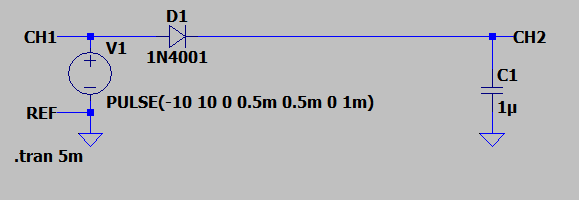
\includegraphics[width=0.8\textwidth]{figures/lab4-3-circuito.PNG}
    \caption{Terceiro circuito simulado no LTSpice.}
    \label{fig:figures-lab4-3-circuito-png}
\end{figure}

Após isso, foi realizada a simulação com resultado apresentado no gráfico mostrado na figura \ref{fig:figures-lab4-3-grafico-png}.

\begin{figure}[H]
    \centering
    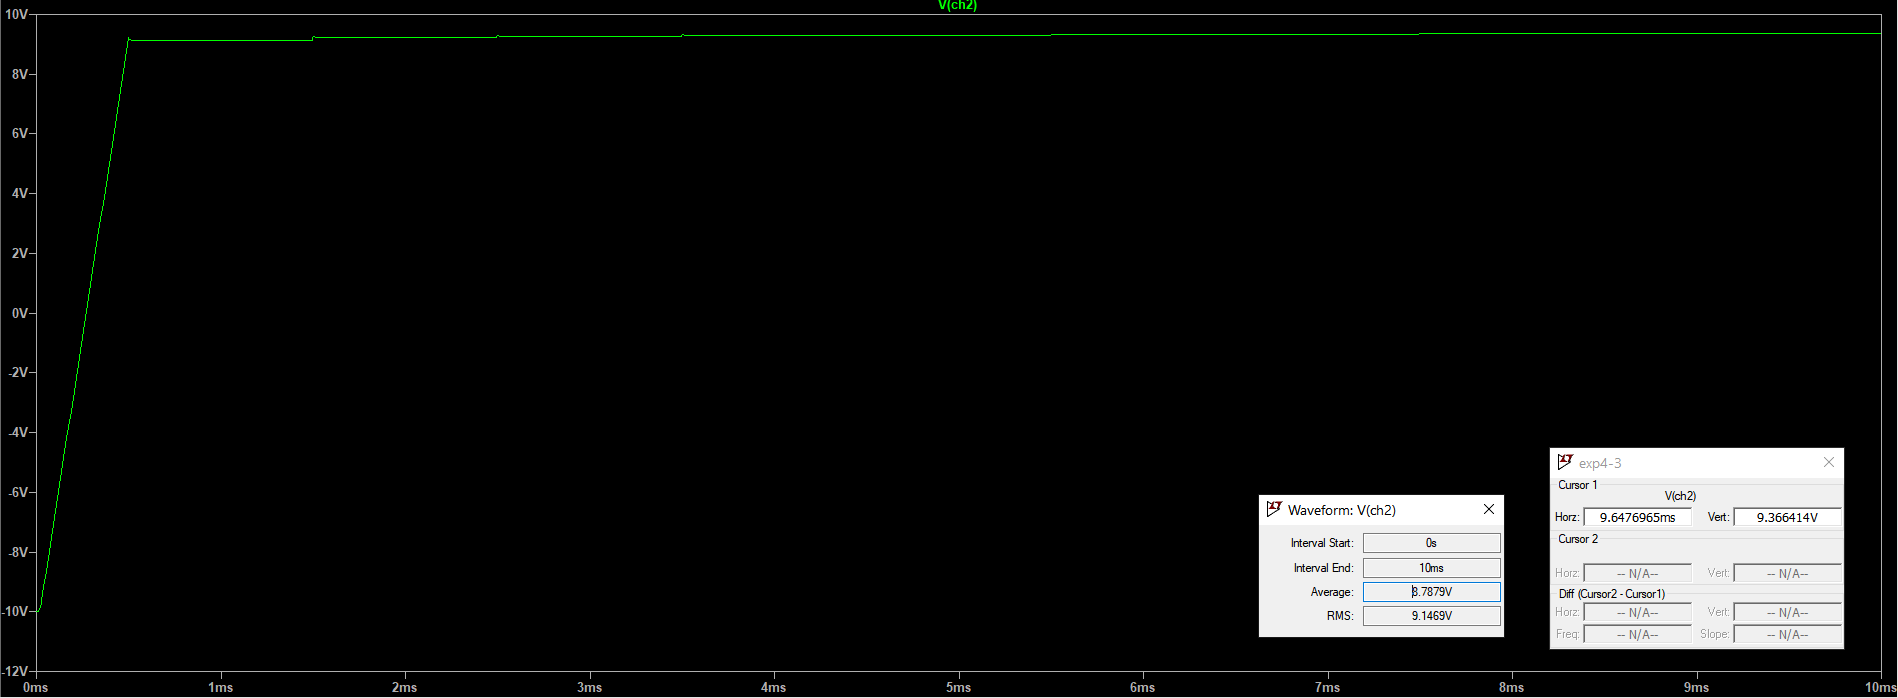
\includegraphics[width=0.8\textwidth]{figures/lab4-3-grafico.PNG}
    \caption{Resposta de $V_o$ no tempo na simulação do LTspice.}
    \label{fig:figures-lab4-3-grafico-png}
\end{figure}

Como mostrado no gráfico acima, o valor de $V_o$ sobe lentamente ao decorrer dos ciclos. Considerando o tempo de 10ms simulado, temos $V_{i,p} \approx 9,36V$ e $V_{o,med} \approx 8,79V$.

\subsection{Circuito 4}

O resultado das medições feitas no circuito simulado pode ser observado na figura \ref{fig:figures-lab4-4-png} e na tabela posterior.

\begin{figure}[H]
    \centering
    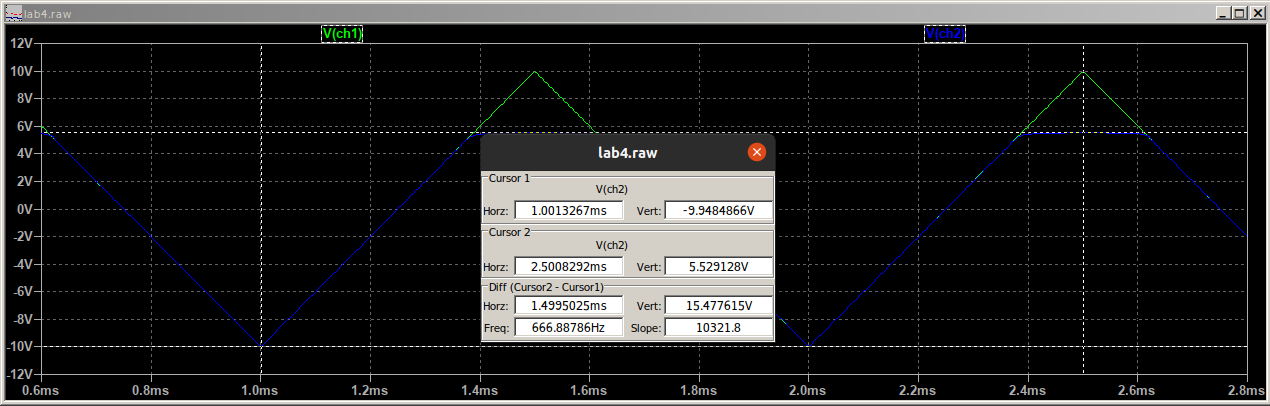
\includegraphics[width=0.8\textwidth]{figures/lab4-4.png}
    \caption{Medição realizada em $V_o$ utilizando as ferramentas do LTSpice.}
    \label{fig:figures-lab4-4-png}
\end{figure}

\begin{table}[H]
    \centering
    \begin{tabular}{c | c}
	Medida & Resultado \\
	\hline
	$V_{i,pp}$ & 19,98 V \\
	$V_{o,pp}$ & 15,48 V \\
	$V_{o,min}$ & -9,95 V \\
	$V_{o,máx}$ & 5,53 V \\
    \end{tabular}
\end{table}

O comportamento da tensão de saída pode ser compreendido em dois momentos. Quando a tensão de entrada $V_i$ é menor do que a tensão $V_x$ somada da queda de tensão do diodo, não há corrente e, portanto, não há queda sobre o resistor $R_1$, logo, $V_o = V_i$. Quando $V_i$ é maior do que $V_x$ somada à queda do diodo, então há uma corrente no circuito e, portanto, o diodo sofre a queda de tensão que, pela malha interna formada, é equivalente à diferença entre a tensão de entrada e a tensão de referência ($V_x$ + diodo), logo, a tensão de saída satura na tensão de referência.

\section*{Conclusão}

Durante a execução do experimento, foi possível perceber as principais características de comportamento do diodo estudado alimentado por uma onda triangular. Além disso, também foi possível comparar esse valor com equações aproximadas, comprovando que os resultados realmente eram próximos.

Por fim, também foram utilizadas novas ferramentas para análise de gráficos no LTspice. As funções utilizadas desenvolveram mais familiaridade com o \textit{software} e devem ser utilizadas nos próximos experimentos.
\end{document}
